
% !TeX document-id = {d8b4925c-2057-42a4-b894-2f1a3f1b6345}
%!TeX TXS-program:compile = txs:///xelatex/[--shell-escape]
\documentclass[aspectratio=169, mathserif]{beamer}% TPU recommends 16:9 ratio, 4:3 may require some work with inner theme .sty file

% Style options:
% light --- light theme (default)
% dark --- dark theme
% enlogo --- english TPU logo {default}
% rulogo --- russian TPU logo

\usetheme[light, rulogo]{tpu}% dark theme used as an example of optional argument

\usepackage[russian]{babel}%uncomment this to work in russian
\usepackage[utf8]{inputenc}

\usepackage{fontspec}

\setromanfont{Brygada1918}[
Path=./fonts/BrygadaFontFiles/,
Extension = .ttf,
UprightFont=*-Regular,
BoldFont=*-Bold,
ItalicFont=*-Italic,
BoldItalicFont=*-BoldItalic
]

\setsansfont{ALSSirius}[
Path=./fonts/ALSSiriusFiles/,
Extension = .otf,
UprightFont=*-Regular,
BoldFont=*-Bold,
%ItalicFont=*-Italic,
%BoldItalicFont=*-BoldItalic
]

\setmonofont{Consolas}[
Path=./fonts/ConsolasFontFiles/,
%Scale=0.85,
Extension = .ttf,
UprightFont=*-Regular,
BoldFont=*-Bold,
ItalicFont=*-Italic,
BoldItalicFont=*-BoldItalic
]

\usepackage[cache=false]{minted}
\usepackage{xcolor} % to access the named colour LightGray
\definecolor{LightGray}{gray}{0.9}
\definecolor{onedarkBckGr}{RGB}{40, 44, 52}

\usemintedstyle[python]{default}
\setminted[python]{
fontsize=\scriptsize,
escapeinside=||,
mathescape=true,
numbersep=5pt,
gobble=2,
linenos=false,
frame=single,
framesep=1mm,
python3=true,
bgcolor=backcolour,
}

\usemintedstyle[pycon]{default}
\setminted[pycon]{
	fontsize=\scriptsize,
	escapeinside=||,
	mathescape=true,
	numbersep=5pt,
	gobble=2,
	linenos=false,
	frame=single,
	framesep=1mm,
	python3=true,
	bgcolor=backcolour,
	linenos=true,
}

\newmint{python}{}

\usepackage{booktabs}% good looking tables
\usepackage{multicol}% text in multiple columns, useful for side-by-side text and pictures
\usepackage{hyperref}
\definecolor{maroon}{cmyk}{0, 0.87, 0.68, 0.32}
\definecolor{halfgray}{gray}{0.55}
\definecolor{ipython_frame}{RGB}{207, 207, 207}
\definecolor{ipython_bg}{RGB}{247, 247, 247}
\definecolor{ipython_red}{RGB}{186, 33, 33}
\definecolor{ipython_green}{RGB}{0, 128, 0}
\definecolor{ipython_cyan}{RGB}{64, 128, 128}
\definecolor{ipython_purple}{RGB}{170, 34, 255}
\definecolor{linkcolor}{HTML}{0000FF} % цвет гиперссылок
\definecolor{urlcolor}{HTML}{800080} % цвет ссылок
\definecolor{backcolour}{rgb}{0.95,0.95,0.92}

\usepackage{longtable}
\usepackage{wrapfig}
\usepackage{ragged2e}
\usepackage[nooneline]{caption}
\DeclareCaptionTextFormat{center}{\centering{#1}}
\captionsetup[table]{justification=raggedleft, 
labelformat=empty,
labelsep=endash,  
textformat=center, 
position=top, 
skip=5pt
}

\hyphenpenalty=10000% i don’t think hyphenation in presentations is a good idea, feel free to change however you like

\title{\LARGE{Системный анализ процессов химической технологии}}
\subtitle{Лекция 2 \\ Структуры данных: \\ строки, списки, кортежи, словари и множества}
\author[]{Вячеслав Алексеевич Чузлов, \\
к.т.н., доцент ОХИ ИШПР}
\date{\today}

\begin{document}

\newcommand{\pythoninline}[1]{%
	\colorbox{white}{%
		\parbox[b][.6em]{\widthof{\mintinline[fontsize=\tiny]{ipython}{#1}}}{\mintinline[fontsize=\tiny]{ipython}{#1}}%
	}%
}

% notice usage of \titleframe and several other unconventional functions
% the reason being is custom backgrounds on these slides

\titleframe% title

\tocframe{}% this custom frame accepts options for ToC



\section{Строки в Python}
\sectionframe


\begin{frame}[fragile]{Основы строк}

\begin{itemize}
\scriptsize
\item Строки в Python относятся к \textcolor{extraorange}{\textbf{неизменяемым последовательностям}}, что говорит о том, что содержащиеся в них символы имеют позиционный порядок слева направо и не могут быть изменены на месте.

\item Строки в Python исполняют ту же роль, что и массивы символов в С-подобных языках, но в сравнении с массивами, они обладают инструментарием более высокого уровня. 

\item Строки в Python снабжены мощным набором инструментов обработки. Кроме того, в отличие от языков, подобных С, в Python не предусмотрен отдельный тип для индивидуальных символов, вместо этого применяются односимвольные строки.

\item В плане обработки строки поддерживают операции \textcolor{extraorange}{\textbf{выражений}}, такие как конкатенация (объединение строк), срезы (извлечение частей), индексация и т.д. Кроме операций выражений Python предоставляет набор \textcolor{extraorange}{\textbf{методов}} строк, которые реализуют общие задачи, специфичные для строк.
\end{itemize}

\vfill
\end{frame}

\subsection{Синтаксис строк}
\begin{frame}[fragile]{Синтаксис строк}
\scriptsize
Python предлагает довольно обширный набор инструментов для работы со строками и в большинстве случаев использование строк проходит довольно легко. Вот несколько возможных способов записи строк в Python-коде:

\begin{itemize}
\item одинарные кавычки~--  \mintinline[style=default]{python}|'spa"m'|;
\item двойные кавычки~-- \mintinline[style=default]{python}|"spa'm"|;
\item тройные кавычки (\textcolor{extraorange}{\textbf{строки документации}})~-- \mintinline[style=default]{python}|"""... spam ..."""|;
\item неформатированные строки~-- \mintinline[style=default]{python}|r'C:\new\test.spm'|;
\item прочие способы записи строк.
\end{itemize}

Формы с одинарными и двойными кавычками, безусловно, являются наиболее популярными, другие используются в особых случаях.
\vfill
\end{frame}


\begin{frame}[fragile]{Строки в одинарных и двойных кавычках}
\scriptsize
Символы одинарных и двойных кавычек имеют одинаковое значение~-- обе формы записи работают абсолютно одинаково и возвращают объект одного типа:
\begin{minted}{pycon}
>>> 'compounds', "compounds"
('compounds', 'compounds')
\end{minted}

Можно внедрять символ одинарной кавычки в строку, заключенную в символы двойной кавычки, и наоборот:
\begin{minted}[firstnumber=last]{pycon}
>>> 'compound"s', "compound's"
('compound"s', "compound's")
\end{minted}

При необходимости можно также внедрять символы кавычек, экранируя их при помощи обратной косой черты:
\begin{minted}[firstnumber=last]{pycon}
>>> 'knight\'s', "knight\"s"
("knight's", 'knight"s')
\end{minted}
\vfill
\end{frame}


\subsection{Операции над строками}

\begin{frame}[fragile]{Операции над строками}
\scriptsize
\begin{enumerate}
\item Встроенная функция \mintinline{python}|len()| возвращает длину строки:
\begin{minted}{pycon}
>>> len('abc')
3
\end{minted}
\item \textcolor{extraorange}{\textbf{Конкатенация}} (сложение) строк выполняется при помощи операции \mintinline{python}|+| и создает новый объект строки с объединенным содержимым ее операндов:
\begin{minted}[firstnumber=last]{pycon}
>>> 'abc' + 'def'
'abcdef'
\end{minted}
\item Повторение выполняется при помощи операции \mintinline{python}|*| и идентично добавлению строки к самой себе несколько раз:

\begin{minted}[firstnumber=last]{pycon}
>>> 'Hi!' * 4  # Повторение: то же, что 'Hi!' + 'Hi!' + ... 
'Hi!Hi!Hi!Hi!'
\end{minted}
\end{enumerate}
\vfill
\end{frame}


\begin{frame}[fragile]{Операции над строками}
\scriptsize
Например, можно вывести на экран формулу \textbf{н-декана}, используя операции конкатенации и повторения:
\begin{minted}{pycon}
>>> 'CH3-' + 'CH2-' * 8 + 'CH3'  
'CH3-CH2-CH2-CH2-CH2-CH2-CH2-CH2-CH2-CH3'
\end{minted}

Для того, чтобы вывести формулу без кавычек, можно использовать встроенную функцию \mintinline{python}|print()|:

\begin{minted}[firstnumber=last]{pycon}
>>> nC10 = 'CH3-' + 'CH2-' * 8 + 'CH3'

>>> print(nC10) 
CH3-CH2-CH2-CH2-CH2-CH2-CH2-CH2-CH2-CH3
\end{minted}
\vfill
\end{frame}


\subsection{Операции индексации и среза}
%\sectionframe


\begin{frame}[fragile]{Операции индексации}
\scriptsize
\begin{itemize}
\item Строки являются упорядоченными коллекциями символов и поэтому поддерживают доступ к своим элементам по индексу.

\item \textcolor{extraorange}{\textbf{Индексация}}~-- предоставление индекса желаемого компонента в квадратных скобках после имени, с которым связан объект строки. Результатом будет являться односимвольная строка в указанной позиции.

\item Индексы в Python начинаются с 0 и заканчиваются величиной, на единицу меньше, чем длина строки. 

\item Python разрешает получать элементы из последовательностей с использованием \textcolor{extraorange}{\textbf{отрицательных}} индексов.
\end{itemize}

\centering
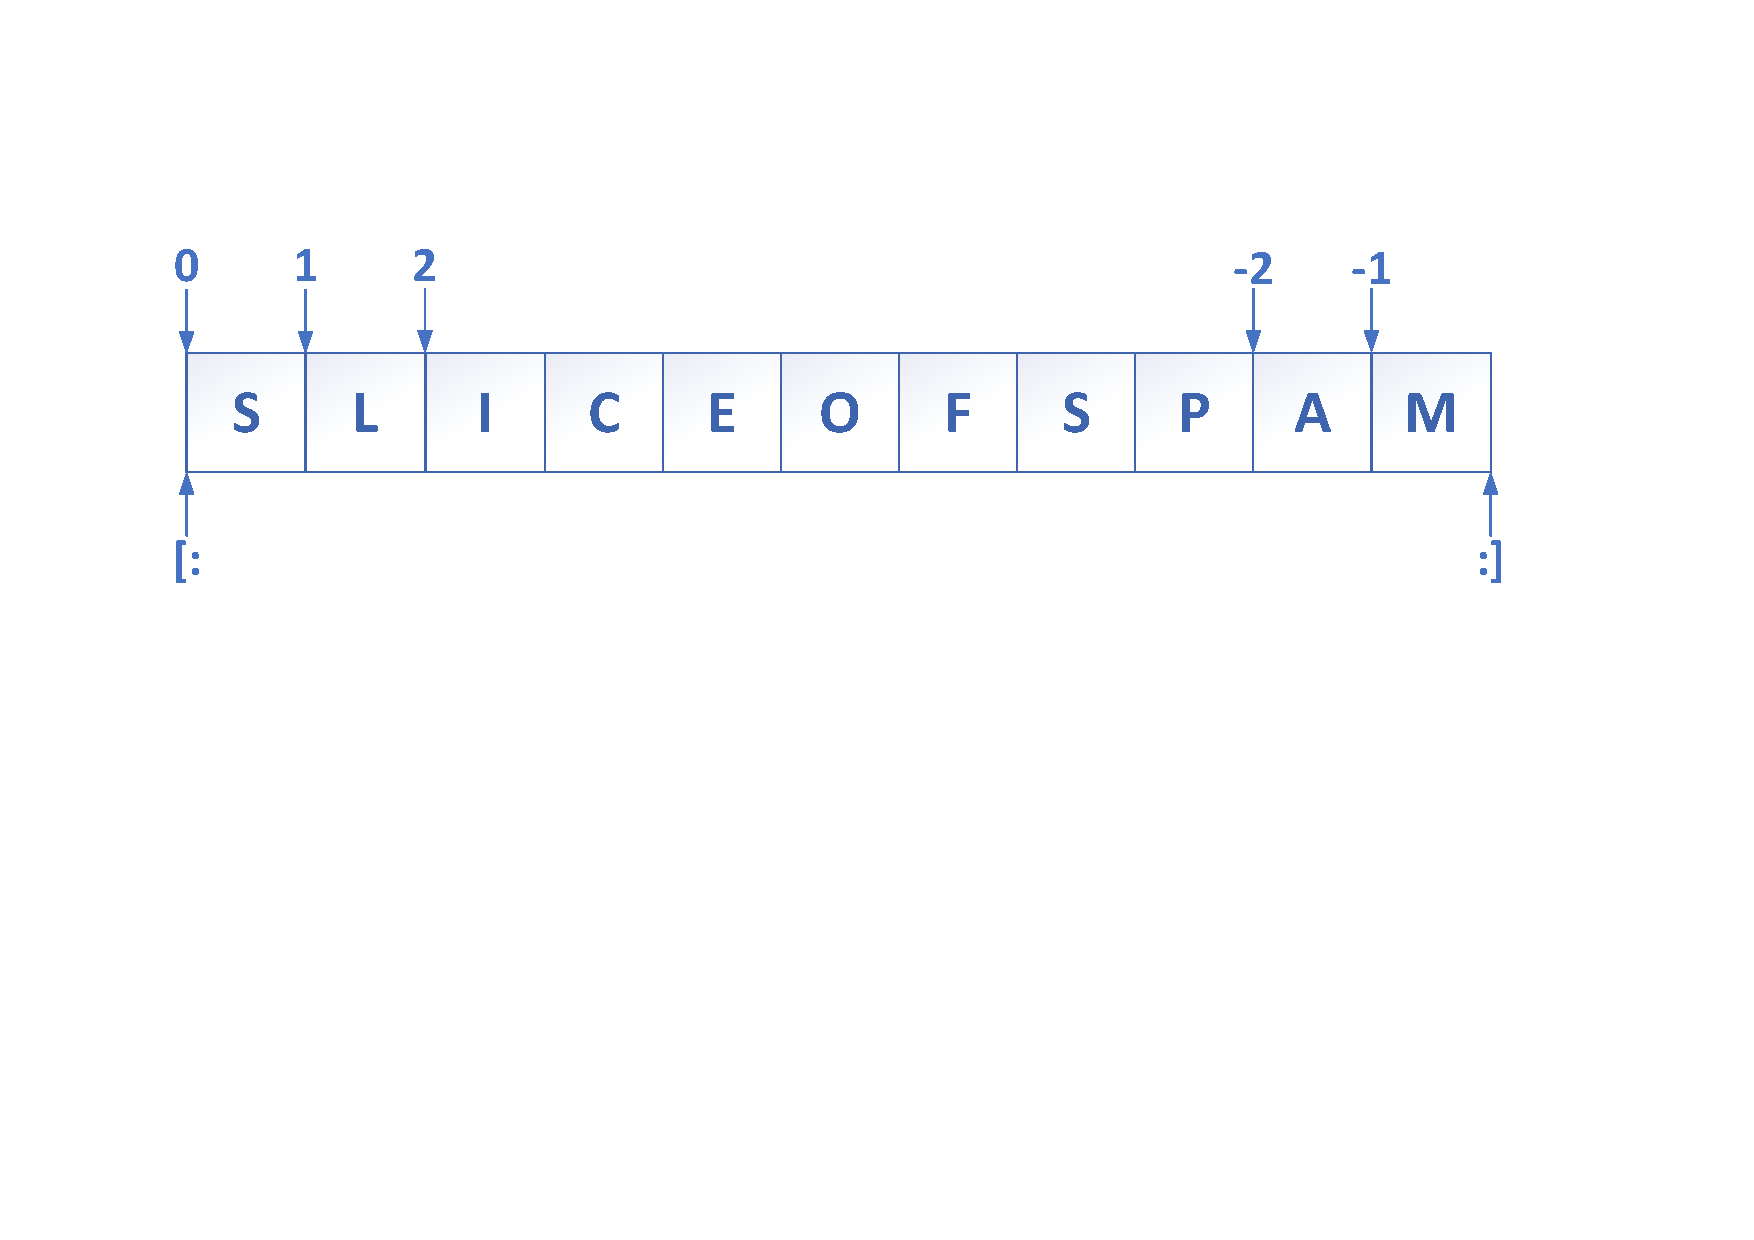
\includegraphics[width=.75\linewidth]{pics/индексы_и_срезы}

\end{frame}


\begin{frame}[fragile]{Операции индексации}

\begin{minted}{pycon}
>>> s = 'chemistry'

>>> s[1], s[-2]
('h', 'r')

>>> for i in range(len(s)):
...     print(s[i].upper())
...
C
H
E
M
I
S
T
R
Y
\end{minted}

\vfill
\end{frame}


\begin{frame}[fragile]{Операции срезов}

\scriptsize
\begin{itemize}
\item \textcolor{extraorange}{\textbf{Срезы}}~-- обобщенная форма индексации для получения целого \textcolor{extraorange}{\textbf{сегмента}} вместо одиночного элемента.

\item При выполнении среза Python извлекает элементы, начиная с нижней границы и заканчивая, но не включая верхнюю границу, и возвращает новый объект, содержащий извлеченные элементы.
\item Если левая и/или правая границы не указаны, по умолчанию для них принимаются индексы 0 и длина последовательности, соответственно.
\end{itemize}

\begin{minted}{pycon}
>>> s = 'chemistry'

>>> s[1:3], s[1:], s[:-1]
('he', 'hemistry', 'chemistr')
\end{minted}

\vfill
\end{frame}


\begin{frame}[fragile]{Расширенные срезы}
\scriptsize
\begin{itemize}
\item В Python для выражений срезов есть поддержка опционального третьего индекса, используемого в качестве \textcolor{extraorange}{\textbf{шага}};

\item  Шаг прибавляется к индексу каждого извлеченного элемента.

\item Полная форма среза выглядит следующим образом:
\begin{center}
\mintinline{ipython}|x[i:j:k]|
\end{center}

\noindent что означает <<извлечь элементы из \texttt{x}, начиная с индекса \texttt{i} и заканчивая индексом \texttt{j-1}, с шагом \texttt{k}>>;

\item Третий предел, \texttt{k}, по умолчанию, равен +1 и поэтому все элементы в срезе обычно извлекаются слева направо. Однако если указать явное значение, то можно применить третий предел для пропуска элементов или смены порядка их следования на противоположный.
\end{itemize}
\vfill
\end{frame}


\begin{frame}[fragile]{Расширенные срезы}
\scriptsize
\begin{itemize}
\item Например, \mintinline{python}|x[1:10:2]| вернет \textcolor{extraorange}{\textbf{каждый второй элемент}} из \mintinline{python}|x| в рамках индексов 1-9, т.е. элементы с индексами 1, 3, 5, 7 и 9. 

\item По аналогии, верхний и нижний пределы по умолчанию принимаются равными 0 и длине последовательности, соответственно, поэтому \mintinline{python}|x[::2]| вернет каждый второй элемент с начала и до конца последовательности:
\end{itemize}

\begin{minted}{pycon}
>>> s = 'Beautifulisbetterthanugly'

>>> s[1:10:2]  # Пропуск элементов
'euiui'

>>> s[::2]
'Batflsetrhngy'

>>> s = 'spam'  

>>> s[::-1]  # Смена порядка  элементов на противоположный 
'maps'
\end{minted}
\vfill
\end{frame}


\begin{frame}[fragile]{Форматированные строки (f-строки)}
\scriptsize
\begin{itemize}
\item Литерал форматированных строк или f-строки~-- это строковый литерал с префиксом \texttt{f} или \texttt{F}. Данные строки могут содержать замещающие поля, которые являются выражениями в фигурных скобках \mintinline{python}|{}|.

\item Мини-язык для спецификатора формата такой же, как и в методе \mintinline{python}|format()|.
\end{itemize}

\begin{minted}{pycon}
>>> f'{1.2354:.2f}'
'1.24'

>>> f'{1.2354:e}'
'1.235400e+00'

>>> f'{1.2354:.3e}'
'1.235e+00'

>>> f'{1.2354:g}'
'1.2354'
\end{minted}
\vfill
\end{frame}


\section{Списки}
\sectionframe


\begin{frame}[fragile]{Списки}
\scriptsize
\begin{itemize}
\item Списки в Python~-- наиболее гибкая разновидность объектов упорядоченных коллекций. 

\item Списки могут содержать объекты любого типа: строки, числа или другие списки.  

\item Списки \textcolor{extraorange}{\textbf{можно изменять}} на месте присваиванием по индексам, с использованием срезов, вызвав специальные методы или выполнив оператор удаления. 
\end{itemize}

\begin{table}[h!]
\centering
\tiny
\begin{tabular}{|p{0.52\linewidth}|p{0.44\linewidth}|}
\hline
\textbf{Операция} & \textbf{Описание} \\
\hline
\mintinline{ipython}|a = []| & Пустой список \\
%\hline
\mintinline{ipython}|a = [123, 'abc', 1.354, []]| & Четыре элемента: индексы 0...3 \\
%\hline
\mintinline{ipython}|a = ['Joe', 30.0, ['dev', 'prof']]| & Вложенные списки \\
%\hline
\mintinline{ipython}|a = list('hello')| & Список элементов итерируемого объекта \\
%\hline
\mintinline{ipython}|a = list(range(-5, 6))| & Список последовательных целых чисел \\
%\hline
\mintinline{ipython}|a[i]| & Индекс \\
%\hline
\mintinline{ipython}|a[i][j]| & Индекс индекса \\
%\hline
\mintinline{ipython}|a[i:j]| & Срез \\
%\hline
\mintinline{ipython}|len(a)| & Длина \\
%\hline
\mintinline{ipython}|a1 + a2| & Конкатенация \\
%\hline
\mintinline{ipython}|a * 3| & Повторение \\
%\hline
\mintinline{ipython}|x in a| & Вхождение \\
%\hline
\mintinline{ipython}|a.append(5)| & Добавление элемента в конец списка \\
%\hline
\mintinline{ipython}|a.extend([10, 20, 30])| & Добавление списка в конец исходного списка \\
\hline
\end{tabular}

\end{table}
\vfill
\end{frame}


\subsection{Базовые операции со списками}

\begin{frame}[fragile]{Базовые операции со списками}
\scriptsize
\begin{itemize}
\item Списки являются \textcolor{extraorange}{\textbf{последовательностями}}, поэтому поддерживают многие операции, характерные для строк. 

\item Например, для списков определены операторы \pythoninline{+} и \pythoninline{*}. Данные операторы, также как и в случае со строками, означают конкатенацию и повторение, только возвращают в качестве результата новый список, а не строку.
\end{itemize}

\begin{minted}{pycon}
>>> len([1, 2, 3, 4, 5])                # Длина
5

>>> [1, 2, 3, 4, 5] + [6, 7, 8, 9, 10]  # Конкатенация
[1, 2, 3, 4, 5, 6, 7, 8, 9, 10]

>>> ['Hi!'] * 5                         # Повторение
['Hi!', 'Hi!', 'Hi!', 'Hi!', 'Hi!']
\end{minted}
\vfill
\end{frame}


\subsection{Итерация по спискам и генераторы списков}

\begin{frame}[fragile]{Итерация по спискам}
\scriptsize
В общем смысле для списков определены все операции над последовательностями, в том числе и инструменты итерации:

\begin{minted}{pycon}
>>> 'banana' in ['banana', 'orange', 'apple']   # Проверка вхождения
True

>>> for fruit in ['banana', 'orange', 'apple']: # Итерация
...     print(fruit, end=' ')
...
banana orange apple
\end{minted}

Оператор цикла \mintinline{python}|for| проходит (итерируется) по всем элементам в любой последовательности (итерируемом объекте) слева направо, выполняя операторы для каждого из них.
\vfill
\end{frame}


\begin{frame}[fragile]{Генераторы списков (list comprehension)}
\scriptsize
\textcolor{extraorange}{\textbf{Генераторы списков}}~-- это способ создания нового списка с применением выражения к каждому элементу последовательности (по факту в любом итерируемом объекте).

\begin{minted}{pycon}
>>> res = [c * 4 for c in 'HELLO']

>>> res
['HHHH', 'EEEE', 'LLLL', 'LLLL', 'OOOO']
\end{minted}

\begin{itemize}
\item Генераторы списков записываются более кратко и выполняются чуть быстрее.

\item В сложных случаях лучше использовать цикл \mintinline{python}|for| из-за его более высокой читаемости.
\end{itemize}

\begin{minted}[firstnumber=last]{pycon}
>>> res = []

>>> for c in 'HELLO':
...     res.append(c * 4)
...

>>> res
['HHHH', 'EEEE', 'LLLL', 'LLLL', 'OOOO']
\end{minted}
\vfill
\end{frame}


\subsection{Индексация, срезы и вложенность}

\begin{frame}[fragile]{Индексация и срезы}
\scriptsize
\begin{itemize}
\item Индексация  и срезы для списков работают аналогично тому, как это было описано для объектов строк. 

\item Результатом индексации списка может быть объект любого типа, находящийся по указанному индексу, тогда как  срезы всегда возвращают новый объект списка.


\begin{minted}{pycon}
>>> fruits = ['banana', 'orange', 'apple']

>>> fruits[2]            # Индексы начинаются с нуля
'apple'

>>> fruits[-2]           # Отрицательные индексы отсчитываются справа
'orange'

>>> fruits[1:3]          # Срезы получают сегменты
['orange', 'apple']

>>> fruits[-1]           # Результат среза всегда новый список
['apple']
\end{minted}
\end{itemize}
\vfill
\end{frame}


\begin{frame}[fragile]{Вложенность списков}
\scriptsize
\begin{itemize}
\item Внутри списков могут содержаться вложенные списки или объекты других типов.
\item Матрицы в Python можно представить в виде вложенных списков.
Пример матрицы $3 \times 3$:

\begin{minted}{pycon}
>>> matrix = [[10, 20, 30], [40, 50, 60], [70, 80, 90]]
\end{minted}
\item Если указать один индекс, то будет получена целая строка, а при указании двух индексов будет возвращен элемент строки:

\begin{minted}[firstnumber=last]{pycon}
>>> matrix[1]
[40, 50, 60]

>>> matrix[2][0]
70

>>> matrix = [[10, 20, 30],
...           [40, 50, 60],
...           [70, 80, 90]]

>>> matrix[1][1]
50
\end{minted}
\end{itemize}
\vfill
\end{frame}


\subsection{Изменение списков}

\begin{frame}[fragile]{Изменение списков}
\scriptsize
\begin{itemize}
\item Так как списки~-- \textcolor{extraorange}{\textbf{изменяемый}} тип объектов, для них определены операции, которые могут модифицировать объект списка \textcolor{extraorange}{\textbf{на месте}}.

\item Операции модифицирования списков изменяют объект списка напрямую, перезаписывая его старое значение, без необходимости создания новой копии, как в случае работы со строками.
\end{itemize}

\alert{\textbf{Присваивание по индексам и срезам}}
\\
Содержимое списка может быть изменено присваиванием значения либо отдельному элементу (по его индексу), либо целому сегменту (по срезу):

\begin{minted}{pycon}
>>> food = ['burger', 'pizza', 'buritto']

>>> food[1] = 'toast'  # Присваивание по индексу

>>> food
['burger', 'toast', 'buritto']

>>> food[:2] = ['need', 'more']  # Присваивание срезу

>>> food
['need', 'more', 'buritto']
\end{minted}
\vfill
\end{frame}


\subsection{Вызовы методов списков}

\begin{frame}[fragile]{Вызовы методов списков}
\scriptsize
\begin{itemize}
\item Подобно строкам, списки имеют набор специфичных методов, многие из которых ведут к изменению исходного списка на месте:
\begin{minted}{pycon}
>>> a = ['eat', 'more', 'SPAM']

>>> a.append('please')

>>> a
['eat', 'more', 'SPAM', 'please']

>>> a.sort()  # Сортировка элементов списка ('S' < 'e')
   
>>> a
['SPAM', 'eat', 'more', 'please']
\end{minted}
\item Наиболее распространенный метод~-- \mintinline{python}|append()| добавляет объект в конец списка. 
\item Эффект выполнения выражения \mintinline{python}|a.append(x)| аналогичен \mintinline{python}|a + [x]| с одним принципиальным отличием: первый вариант изменяет \texttt{a} на месте, а второй вариант создает новый объект списка. 
\item Метод \mintinline{python}|sort()| упорядочивает элементы в списке.
\end{itemize}
\vfill
\end{frame}

\begin{frame}[fragile]{Дополнительные сведения о методе \texttt{sort()}}
\scriptsize
\begin{itemize}
	\item В методе \mintinline{python}|sort()| аргумент \mintinline{python}|reverse| позволяет производить сортировку в порядке убывания вместо возрастания, а параметр \mintinline{python}|key| задает функцию с одним аргументом, которая возвращает значение для использования при сортировке.
\begin{minted}[fontsize=\fontsize{8pt}{8pt}]{pycon}
>>> a = ["abc", "ABD", "aBe"]   

>>> a.sort()                             # Сортировка со смешанным регистром

>>> a
['ABD', 'aBe', 'abc']

>>> a = ["abc", "ABD", "aBe"]

>>> a.sort(key=str.lower)                # Приведение к нижнему регистру

>>> a
['abc', 'ABD', 'aBe']

>>> a.sort(key=str.lower, reverse=True)  # Изменение порядка сортировки

>>> a
['aBe', 'ABD', 'abc']
\end{minted}
\end{itemize}
\vfill
\end{frame}


\section{Кортежи}
\sectionframe

\begin{frame}[fragile]{Кортежи}

\scriptsize
\begin{itemize}
\item Кортежи служат для хранения нескольких объектов вместе. 
\item Аналог списков, но без обширной функциональности. Кортежи \textcolor{extraorange}{\textbf{неизменяемы}}.
\end{itemize}

\begin{table}[h!]
\centering
\tiny
\begin{tabular}{|p{0.4\textwidth}|p{0.55\textwidth}|}
\hline
\textbf{Операция} & \textbf{Описание} \\ 
\hline 
\mintinline{ipython}|{t = ()| & Пустой кортеж \\
%\hline
\mintinline{ipython}|t = (0, )| & Одноэлементный кортеж (не выражение) \\
%\hline
\mintinline{ipython}|t = (0, 'Hi', 1.2, 3)| & Кортеж из четырех элементов \\
%\hline
\mintinline{ipython}|t = 0, 'Hi', 1.2, 3| & Такой же кортеж, как в предыдущей строке \\
%\hline
\mintinline{ipython}|t = ('John', ('prof', 'dev'))| & Вложенные кортежи \\
%\hline
\mintinline{ipython}|t = tuple('hello')| & Кортеж из элементов итерируемого объекта \\
%\hline
\mintinline{ipython}|t[i]| & Индекс \\
%\hline
\mintinline{ipython}|t[i][j]| & Индекс индекса \\
%\hline
\mintinline{ipython}|t[i:j]| & Срез \\
%\hline
\mintinline{ipython}|len(t)| & Длина кортежа \\
%\hline
\mintinline{ipython}|t1 + t2| & Конкатенация \\
%\hline
\mintinline{ipython}|t * 3| & Повторение \\
%\hline
\mintinline{ipython}|'spam' in t| & Проверка вхождения\\
%\hline
\mintinline{ipython}|t.index('Hi')| & Поиск индекса элемента \\
%\hline
\mintinline{ipython}|t.count('hello')| & Подсчет повторений элемента \\
%\hline
\hline

\end{tabular}

\end{table}
\vfill
\end{frame}


\subsection{Операции над кортежами}

\begin{frame}[fragile]{Операции над кортежами}
\scriptsize
\begin{itemize}
\item Кортежи поддерживают обычные операции, специфичные для последовательностей:
\begin{minted}[fontsize=\fontsize{7pt}{8pt}]{pycon}
>>> (10, 20) + (30, 40)             # Конкатенация
(10, 20, 30, 40)

>>> (1, 2) * 5                      # Повторение
(1, 2, 1, 2, 1, 2, 1, 2, 1, 2)  

>>> t = (10, 20, 30, 40, 50)

>>> t[0], t[1:3]                    # Индексация, срезы
(10, (20, 30))
\end{minted}
\item Создание кортежа из одного элемента:
\begin{minted}[fontsize=\fontsize{7pt}{7pt}, firstnumber=last]{pycon}
>>> x = (30)     # Целое число

>>> x
30

>>> y = (30, )   # Кортеж, содержащий целое число

>>> y
(30,)
\end{minted}
\end{itemize}
\vfill
\end{frame}


\begin{frame}[fragile]{Преобразование кортежей}
\scriptsize
Изменять элементы кортежей по индексу, как и элементы строк, нельзя:

\begin{minted}{pycon}
>>> t = (1, 2, 3, 4, 5)

>>> t[1] = 'hi!'     
Traceback (most recent call last):
  File "<stdin>", line 1, in <module>
TypeError: 'tuple' object does not support item assignment

>>> s = 'compound'

>>> s[3] = 'b'
Traceback (most recent call last):
  File "<stdin>", line 1, in <module>
TypeError: 'str' object does not support item assignment
\end{minted}
\vfill
\end{frame}


\section{Словари}
\sectionframe

\begin{frame}[fragile]{Словари (\texttt{dict})}
\scriptsize
\begin{itemize}
\item \textbf{Словари} представляют собой  наиболее гибкие структуры данных в Python. Их можно представить как некий аналог адресной книги, в которой можно найти адрес или контактную информацию о человеке, зная лишь его имя. 

\item Словари не сохраняют порядок следования своих элементов в отличие от списков. 

\item Элементы  словарей хранятся и извлекаются по \textcolor{extraorange}{\textbf{ключам}}, а не по индексам. 

\item Поиск элементов в словаре по ключу является крайне быстрой операцией, т.к. сами словари представляют собой максимально оптимизированную структуру данных.

\end{itemize}

\begin{table}[h!]
\centering
\scriptsize
\begin{tabular}{|p{0.54\textwidth}|p{0.4\textwidth}|}
	\hline
	\textbf{Операция} & \textbf{Интерпретация} \\
	\hline
	\texttt{d = \{\}} & Пустой словарь \\
	\texttt{d = \{\textcolor{ipython_red}{'name'{}}: \textcolor{ipython_red}{'John'{}}, \textcolor{ipython_red}{'age'{}}: 35\}} & Словарь из двух элементов \\
	\texttt{d1 = \{\textcolor{ipython_red}{'person'{}}: \{\textcolor{ipython_red}{'name'{}}: \textcolor{ipython_red}{'John'{}}, \textcolor{ipython_red}{'age'{}}: 35\}\}} & Вложенный словарь	 \\
	\texttt{d = dict(name=\textcolor{ipython_red}{'John'{}}, age=35)} & Создание словаря по ключевым словам \\
	\texttt{d = dict([(\textcolor{ipython_red}{'name'{}}, \textcolor{ipython_red}{'John'{}}), (\textcolor{ipython_red}{'age'{}}, 40)])} & Создание словаря по парам <<ключ: значение>> \\
	%	\texttt{d = dict(zip(keyslist, valueslist))} & Создание словаря по упакованным парам <<ключ: значение>> \\
	\texttt{d = dict.fromkeys([\textcolor{ipython_red}{'name'{}}, \textcolor{ipython_red}{'age'{}}])} & Создание словаря по списку ключей \\
	\texttt{d[\textcolor{ipython_red}{'name'{}}]} & Индексирование по ключу \\
	\texttt{d1[\textcolor{ipython_red}{'person'{}}][\textcolor{ipython_red}{'age'{}}]} & Индексирование по ключу дважды для доступа к вложенным объектам \\
	\texttt{\textcolor{ipython_red}{'age'{}} \textcolor{ipython_green}{in} d} & Проверка наличия ключа \\
	\hline
	
\end{tabular}

\end{table}
\vfill
\end{frame}


\subsection{Базовые операции со словарями}

\begin{frame}[fragile]{Базовые операции со словарями}
\scriptsize
\begin{itemize}
\item Обычно сначала создается словарь при помощи литерального выражения, а затем в нем сохраняются элементы, доступ к которым в последствии производится по ключам:

\begin{minted}{pycon}
>>> d = {'spam': 3, 'ham': 2, 'eggs': 4}  # Создание словаря

>>> d['spam']  # Получение значения по ключу
3

>>> d  # Порядок может измениться
{'spam': 3, 'ham': 2, 'eggs': 4}  
\end{minted}

\item Для индексации словарей применяется тот же синтаксис с квадратными скобками, что и для списков, однако в данном случае он означает доступ по ключу, а не по индексу.
\end{itemize}
\vfill
\end{frame}


\begin{frame}[fragile]{Базовые операции со словарями}
\scriptsize
\begin{itemize}
\item Встроенная функция \pythoninline|len| работает со словарями также, как со списками и строками~-- возвращает количество элементов, хранящихся в словаре или длину списка его ключей. 

\item Операция проверки вхождения \pythoninline|in| в случае со словарями позволяет проверять существование ключей, а метод \pythoninline|keys()| возвращает все ключи:

\begin{minted}[firstnumber=last]{pycon}

>>> len(d)               # Количество элементов в словаре
3

>>> 'eggs' in d          # Проверка вхождения
True

>>> list(d.keys())       # Создание списка ключей в словаре d
['spam', 'ham', 'eggs']
\end{minted}

\item Вызов метода \mintinline{python}|keys()| помещен внутрь функции \mintinline{python}|list()|, по причине того, что метод \mintinline{python}|keys()| возвращает итератор вместо физического списка. Вызов функции \mintinline{python}|list()| получает все значения этого итератора и сохраняет их, хотя в ряде случаев использование списков не требуется.
\end{itemize}
\vfill
\end{frame}

\subsection{Изменение словарей}
\scriptsize
\begin{frame}[fragile]{Изменение словарей}
\begin{itemize}
\item Наряду со списками, словари являются \textcolor{extraorange}{\textbf{изменяемыми}} объектами.
\item  Для изменения или создания элемента нужно выполнить присваивание по ключу. 
\item Оператор \mintinline{python}|del| производит удаление элемента по ключу.

\begin{minted}{pycon}
>>> d = {'spam': 3, 'ham': 2, 'eggs': 4}

>>> d['ham'] = ['grill', 'bake', 'fry']   # Замена значения на список

>>> d
{'spam': 3, 'ham': ['grill', 'bake', 'fry'], 'eggs': 4}

>>> del d['spam']  # Удаление элемента

>>> d
{'ham': ['grill', 'bake', 'fry'], 'eggs': 4}

>>> d['brunch'] = 'Bacon'  # Добавление нового элемента

>>> d
{'ham': ['grill', 'bake', 'fry'], 'eggs': 4, 'brunch': 'Bacon'}
\end{minted}
\end{itemize}
\vfill
\end{frame}

\subsection{Вложенные словари}

\begin{frame}[fragile]{Вложенные словари}
\scriptsize
\begin{itemize}
\item Словари позволяют представлять \textcolor{extraorange}{\textbf{структурированную}} информацию.

\begin{minted}{pycon}
>>> data = {'name': 'John',
...         'jobs': ['developer', 'professor'],
...         'web': 'www.john.org/john',
...         'home': {'state': 'Overworked', 'zip': 13546}}
\end{minted}
\item Для доступа к вложенным объектам нужна цепочка операций индексирования:

\begin{minted}[firstnumber=last]{pycon}
>>> data['name']
'John'

>>> data['jobs']
['developer', 'professor']

>>> data['jobs'][1]
'professor'

>>> data['home']['state']
'Overworked'
\end{minted}
\end{itemize}
\vfill
\end{frame}

\subsection{Инициализация словарей}

\begin{frame}[fragile]{Инициализация словарей}
\scriptsize
В качестве иллюстрации  стандартного способа инициализации словаря, рассмотрим объединение его ключей и значений при помощи функции \mintinline{python}|zip()| с последующей передачей результата вызову \mintinline{python}|dict()|:

\begin{minted}{pycon}
>>> list(zip(['a', 'b', 'c'], [1, 2, 3]))  # Упаковка ключей и значений
[('a', 1), ('b', 2), ('c', 3)]

>>> d = dict(zip(['a', 'b', 'c'], [1, 2, 3]))

>>> d
{'a': 1, 'b': 2, 'c': 3}
\end{minted}
\vfill
\end{frame}


\subsection{Генераторы словарей}

\begin{frame}[fragile]{Генераторы словарей (dict comprehension)}
\scriptsize
\begin{itemize}
\item Генераторы словарей выполняют подразумеваемый цикл, накапливая на каждом шаге результаты <<ключ: значение>> и используя их для заполнения нового словаря:

\begin{minted}[fontsize=\fontsize{7pt}{8pt}]{pycon}
>>> d = {k: v for k, v in zip(['a', 'b', 'c'], [1, 2, 3])}

>>> d
{'a': 1, 'b': 2, 'c': 3}

>>> d = {x: x ** 2 for x in [1, 2, 3, 4, 5]}

>>> d
{1: 1, 2: 4, 3: 9, 4: 16, 5: 25}

>>> d = {c: c * 5 for c in 'hello'}

>>> d
{'h': 'hhhhh', 'e': 'eeeee', 'l': 'lllll', 'o': 'ooooo'}

>>> fruits = {fruit.upper(): fruit + '!' 
...           for fruit in ['banana', 'orange', 'apple']}

>>> fruits
{'BANANA': 'banana!', 'ORANGE': 'orange!', 'APPLE': 'apple!'}
\end{minted}
\end{itemize}
\vfill
\end{frame}


\subsection{Словарные представления}

\begin{frame}[fragile]{Словарные представления}
\scriptsize
\begin{itemize}
\item Методы словарей \mintinline{python}|keys()|, \mintinline{python}|values()| и \mintinline{python}|items()| возвращают \textcolor{extraorange}{\textbf{объекты представлений}}. 

\begin{minted}[fontsize=\fontsize{6.5pt}{7pt}]{pycon}
>>> d = dict(x=1, y=2, z=3)

>>> d
{'x': 1, 'y': 2, 'z': 3}

>>> k = d.keys()

>>> k
dict_keys(['x', 'y', 'z'])

>>> list(k)
['x', 'y', 'z']

>>> v = d.values()

>>> v
dict_values([1, 2, 3])

>>> list(v)
[1, 2, 3]

>>> d.items()
dict_items([('x', 1), ('y', 2), ('z', 3)])

>>> list(d.items())
[('x', 1), ('y', 2), ('z', 3)]
\end{minted}
\end{itemize}
\vfill
\end{frame}


\section{Множества}
\sectionframe

\begin{frame}[fragile]{Множества (\texttt{set})}
	\scriptsize
	\begin{itemize}
		\item \textcolor{extraorange}{\textbf{Множество}} представляет собой неупорядоченную коллекцию \textbf{уникальных} элементов, являющихся  неизменяемыми объектами. 
		\item Элемент встречается во множестве только один раз, в независимости от того, сколько раз он был добавлен.
		\item Поскольку множества представляют собой коллекции других элементов, они разделяют некоторые свойства и поведение с такими типами, как \textbf{списки} и \textbf{словари}. Например, множества являются \textbf{итерируемыми объектами}, их можно увеличивать и уменьшать по требованию, в них можно добавлять объекты других типов.
		
		\item Множества не сохраняют порядок следования элементов и не отображают ключи на значения.
		\item Множества являются \textcolor{extraorange}{\textbf{изменяемыми объектами}} и не могут быть вложенны в другие множества.
	\end{itemize}
	\vfill
\end{frame}


\subsection{Создание объектов множеств}

\begin{frame}[fragile]{Создание объектов множеств}
\scriptsize
\begin{itemize}
\item Для создания объекта множества можно вызвать функцию \pythoninline|set()| и передать ей любой тип последовательности или другой итерируемый объект.
\item В качестве результата будет получен объект множества, содержащий все элементы из переданного объекта (порядок элементов может варьироваться):

\begin{minted}{pycon}
>>> x = set('hello')

>>> x
{'l', 'h', 'e', 'o'}
\end{minted}

\item Для создания объектов множеств  можно также использовать форму литералов множеств, применяя фигурные скобки \pythoninline|{}|. Следующие операторы эквивалентны:

\begin{minted}[firstnumber=last]{pycon}
>>> set([10, 20, 30, 40, 50])
{40, 10, 50, 20, 30}

>>> {10, 20, 30, 40, 50}
{40, 10, 50, 20, 30}
\end{minted}
\end{itemize}
\vfill
\end{frame}

\subsection{Операции над множествами}
\begin{frame}[fragile]{Операции над множествами}
\scriptsize
Созданные объекты множеств поддерживают распространенные математические операции, характерные для множеств:

\centering
\begin{tabular}{cc}
	Объединение & Пересечение \\
	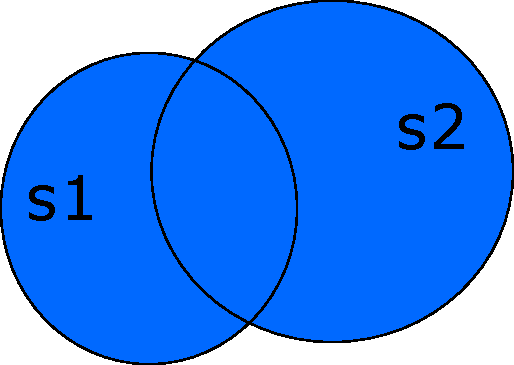
\includegraphics[width=.27\textwidth]{pics/union} &
	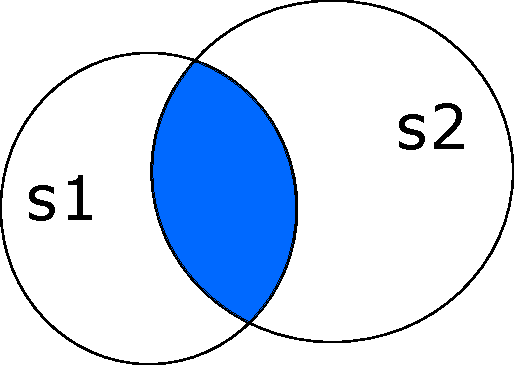
\includegraphics[width=.27\textwidth]{pics/intersection} \\
	Разность & Симметрическая разность \\
	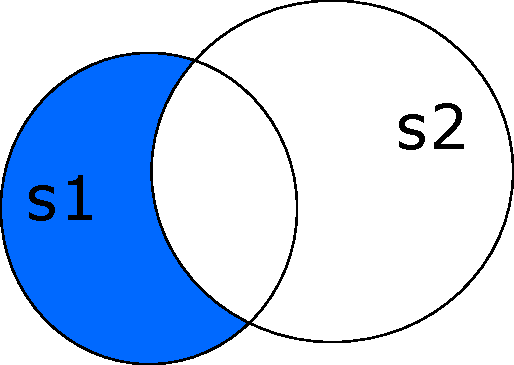
\includegraphics[width=.27\textwidth]{pics/difference} &
	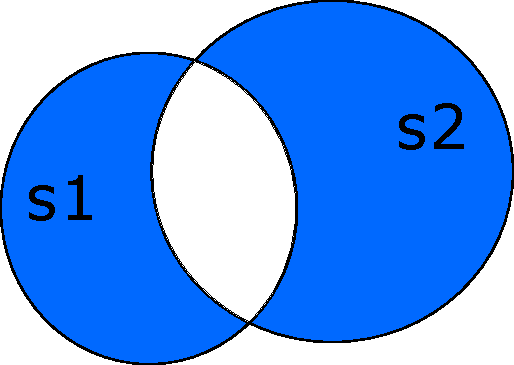
\includegraphics[width=.27\textwidth]{pics/simmetric_difference} \\
\end{tabular}
\vfill
\end{frame}

\begin{frame}[fragile]{Операции над множествами}
\scriptsize
Операторы \textcolor{extraorange}{\textbf{выражений}}, определенные для объектов множеств:

\begin{minted}[escapeinside=//, fontsize=\fontsize{8pt}{8pt}]{pycon}
>>> x = set('hello')

>>> y = set('python')

>>> x - y  # Разность
{'l', 'e'}

>>> x | y  # Объединение
{'l', 'h', 'p', 'y', 't', 'n', 'e', 'o'}

>>> x & y  # Пересечение
{'h', 'o'}

>>> x ^ y  # Симметрическая разность
{'l', 'n', 'p', 'y', 't', 'e'}

>>> x > y, x < y  # Надмножество, подмножество
(False, False)

>>> 'h' in x  # Проверка вхождения во множество
True
\end{minted}
\vfill
\end{frame}

\subsection{Примеры использования множеств}

\begin{frame}[fragile]{Примеры использования множеств}
\scriptsize
\begin{itemize}
\item Поскольку элементы во множестве сохраняются только однократно, множества могут быть использованы для \textcolor{extraorange}{\textbf{фильтрации дубликатов}} в коллекциях. 
\item Коллекцию лишь нужно преобразовать во множество и затем выполнить обратное преобразование (если в этом есть необходимость):

\begin{minted}{pycon}
>>> a = [1, 2, 2, 3, 5, 4, 1, 1, 2, 5, 4]

>>> set(a)
{1, 2, 3, 4, 5}|

>>> a = list(set(a))

>>> a
[1, 2, 3, 4, 5]|

>>> list(set(['hh', 'ee', 'll', 'll', 'oo'])) # Порядок не сохраняется
['oo', 'hh', 'll', 'ee']
\end{minted}
\end{itemize}
\vfill
\end{frame}

\begin{frame}[fragile]{Примеры использования множеств}
	
\begin{itemize}
\item Множества могут также быть использованы при нахождении \textcolor{extraorange}{\textbf{различий}} в списках, строках и прочих итерируемых объектах, однако снова нужно помнить о том, что исходный порядок следования элементов в сравниваемых объектах может быть изменен:

\begin{minted}[firstnumber=last]{pycon}
>>> a = [1, 2, 3, 4, 5, 7]

>>> a2 = [1, 2, 4, 5, 6]

>>> set(a) - set(a2)  # Различия в списках
{3, 7}

>>> s1 = 'spam'

>>> s2 = 'ham'

>>> set(s1) - set(s2)  # Различия в строках
{'s', 'p'}

>>> set('tomato') - set(['p', 'o', 't', 'a', 't', 'o'])  # Объекты разных типов
{'m'}
\end{minted}
\end{itemize}
\vfill
\end{frame}

\begin{frame}[fragile]{Примеры использования множеств}
\scriptsize
\begin{itemize}
\item Множества также можно применить для проверок на \textcolor{extraorange}{\textbf{равенство, нейтральное к порядку}}. 
\item Два множества равны только в том случае, когда каждый элемент одного множества содержится в другом, иначе говоря, одно множество является подмножеством другого. 
\item К примеру, такой прием можно использовать для сравнения выводов программ, которые должны работать одинаковым образом, но могут генерировать результаты в разном порядке:

\begin{minted}[firstnumber=last]{pycon}
>>> a1, a2 = [1, 2, 3, 5, 4, 6], [2, 5, 3, 4, 1, 6]

>>> a1 == a2  # Порядок следования имеет значение
False

>>> set(a1) == set(a2)  # Проверка, нейтральная к порядку элементов
True

>>> 'hello' == 'olleh', set('hello') == set('olleh')
(False, True)
\end{minted}
\end{itemize}
\vfill
\end{frame}


\contactsframe[\Large \textbf{Благодарю за внимание!}]{


\includegraphics[width=.05\textwidth]{pics/home} \quad Учебный корпус №2, ауд. 136 \\

\includegraphics[width=.05\textwidth]{pics/mail} \quad chuva@tpu.ru \\

\includegraphics[width=.03\textwidth]{pics/tel} \quad +7-962-782-66-15
}

\end{document}

